\documentclass{article}
\usepackage[utf8]{inputenc}
\usepackage{tikz}
\usetikzlibrary{external}
\tikzexternalize[mode=list and make]

\tikzset{
    png export/.style={
        % First we call ImageMagick; change settings to requirements
        external/system call/.add={}{; convert -density 300 -transparent white "\image.pdf" "\image.png"},
        % Now we force the PNG figure to be used instead of the PDF
        /pgf/images/external info,
        /pgf/images/include external/.code={
            \includegraphics[width=\pgfexternalwidth,height=\pgfexternalheight]{##1.png}
        },
    }
  }
  
\title{Keane Imai (2004) Figure 1}
\author{John Green }

\date{November 2022}
\begin{document}

{
\tikzset{png export}
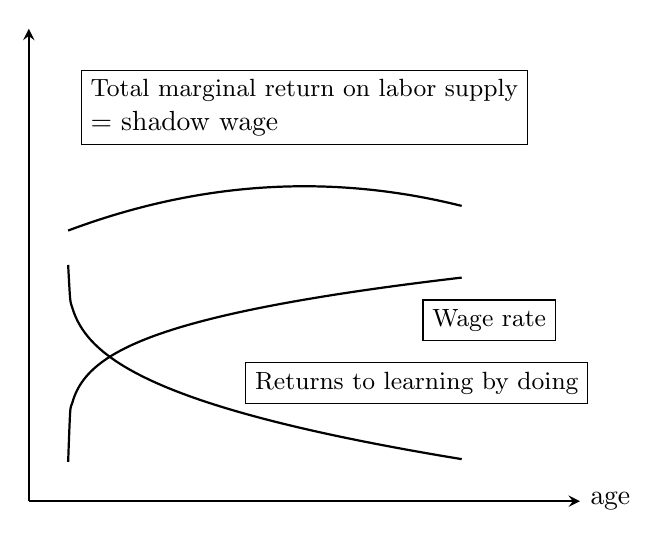
\begin{tikzpicture}
\draw[-stealth, black, thick] (0,0) -- (7,0) node[right] { age};
\draw[-stealth, black, thick] (0,0) -- (0,6);
\draw[thick, smooth, samples=200, xshift=.5cm, yshift=.5cm, domain=0:5] plot ({ \x, {(6*\x)^(1/4)}});
\node[right] at (5,2.3) [rectangle,draw] {\small Wage rate};
\draw[thick, smooth, samples=200, xshift=.5cm, yshift=3cm, domain=0:5] plot ({ \x, {-(3*\x)^(1/3)}});
\node[right] at (2.75,1.5) [rectangle,draw] {\small Returns to learning by doing};
% \draw[thick, smooth, samples=200, xshift=.5cm, yshift=2.5cm, domain=0.05:2.05] plot ({ \x, {\x^(1/2)-\x^(1/3)}});
\draw[thick, smooth, samples=200, xshift=-.5cm, yshift=2cm, domain=1:6] plot ({ \x, {2-(\x/4 - 1)^2}});
\node[align=left] at (3.5,5) [rectangle,draw] {\small Total marginal return on labor supply \\ = shadow wage};
\end{tikzpicture}
}

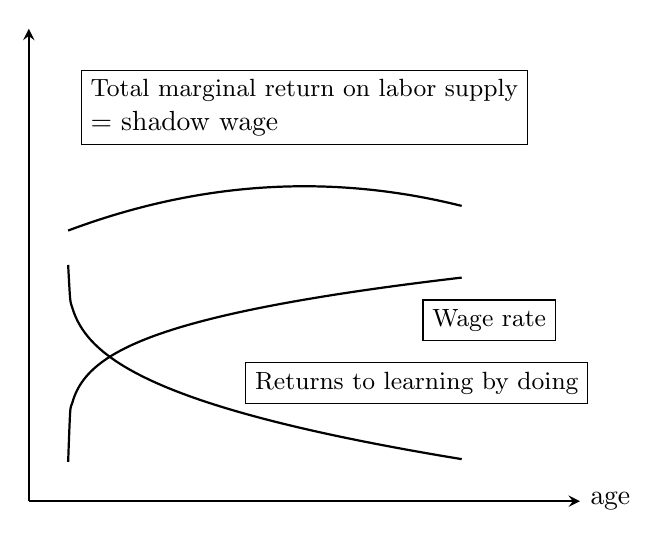
\begin{tikzpicture}
\draw[-stealth, black, thick] (0,0) -- (7,0) node[right] { age};
\draw[-stealth, black, thick] (0,0) -- (0,6);
\draw[thick, smooth, samples=200, xshift=.5cm, yshift=.5cm, domain=0:5] plot ({ \x, {(6*\x)^(1/4)}});
\node[right] at (5,2.3) [rectangle,draw] {\small Wage rate};
\draw[thick, smooth, samples=200, xshift=.5cm, yshift=3cm, domain=0:5] plot ({ \x, {-(3*\x)^(1/3)}});
\node[right] at (2.75,1.5) [rectangle,draw] {\small Returns to learning by doing};
% \draw[thick, smooth, samples=200, xshift=.5cm, yshift=2.5cm, domain=0.05:2.05] plot ({ \x, {\x^(1/2)-\x^(1/3)}});
\draw[thick, smooth, samples=200, xshift=-.5cm, yshift=2cm, domain=1:6] plot ({ \x, {2-(\x/4 - 1)^2}});
\node[align=left] at (3.5,5) [rectangle,draw] {\small Total marginal return on labor supply \\ = shadow wage};
\end{tikzpicture}

\end{document}
